\documentclass[a4paper]{article}
\usepackage[margin=15mm, nohead]{geometry}
%~ \usepackage[T2A]{fontenc}
%~ \usepackage[no-math]{fontspec}
\usepackage[dvipsnames]{xcolor}
\usepackage{calc}
\usepackage{graphicx}
\usepackage{physics}
\usepackage{amssymb}
\usepackage{indentfirst}
\usepackage{accents}
\usepackage[colorlinks=true, linkcolor=purple, citecolor=black, urlcolor=blue]{hyperref}
\usepackage{booktabs}
\usepackage{makecell}
\usepackage{multirow}


%~ \setmainfont[BoldFont=Montserrat Medium]{Montserrat Regular}
\newcommand{\then}{\quad\Rightarrow\quad}
\allowdisplaybreaks
\newcommand{\mts}{{\mathstrut}}
\let\up\uparrow
\let\dn\downarrow




\title{\textbf{ZZ-b method: Phasing stage}}
\author{Michal Hordecki \small (formatting by IliKo) \\
E-mail: \url{mhordecki@gmail.com} \\
Website: \href{https://web.archive.org/web/20090903194420/http://www.emsee.110mb.com/Speedcubing/ZZ\%20speedcubing\%20system.html}{http://www.emsee.110mb.com/Speedcubing}}
\date{13$^\text{th}$ August 2008}

\begin{document}

\maketitle
\thispagestyle{empty}

\section*{Introduction}

Here I describe my phasing method. I use simple blockbuilding consisting of 2 blocks and 2 slots. I do phasing while doing last slot (and I do last slot at the end of F2L).

\smallskip
Virtually all of F2L cases end similarly. It is usually something like U R U' R' or R U R' or R' in special cases. Therefore, while doing 4$^\text{th}$ slot, I recognize phasing situation, and then at the end I apply proper moves.

\smallskip
If you allow AUF after phasing, there are 3 possible LL edges permutation cases for you to recognize.

To simplify explanation, assume that the 4$^\text{th}$ slot is the DFR+FR pair.

\smallskip
To name each case, I use the following approach:

Execute R U' R' on the solved cube. You will end with easy F2L case. When looking at the front of the cube, you can see three LL edges --- one placed in UF, another in UR and the last in FR. By these 3 edges you can recognize phasing situation. At first, notice that within three edges there is always a pair of opposite edges, i.e. UF-UB or UR-UL. I'm recognizing the phasing case by looking where these opposite edges are.

\smallskip
I use 2-letter system: for example x-F means that the opposite edges are placed in FR (x) and UF (F), F-R is UF and UR.

\begin{figure}[htb!]
\centering
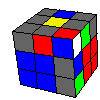
\includegraphics[height=2cm]{Example.png}
\caption{Sample phasing case --- x-R}
\end{figure}

\vfill
\section*{Algorithms}
\vspace{-10pt}

\begin{table}[htb!]
\centering
\def\arraystretch{1.4}
\begin{tabular}{clcr}
Case \hspace{1cm} & Name & Layout & Algorithm
\\ \toprule
\multirow{3}{*}{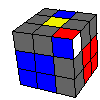
\includegraphics[height=20mm]{RUpRp.png} \hspace{1cm}} & \multirow{3}[3]{*}{R U R' \hspace{1cm}} & x-F & R U' R' U' (R U' R')
\\ \cmidrule{3-4}
& & x-R & (R U2 R' U) (R U2 R')
\\ \cmidrule{3-4}
& & F-R & R U R'
\\ \midrule
\multirow{3}{*}{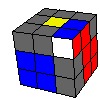
\includegraphics[height=20mm]{URUpRp.png} \hspace{1cm}} & \multirow{3}[3]{*}{U R U' R' \hspace{1cm}} & x-F & U R U' R'
\\ \cmidrule{3-4}
& & x-L & U2 R U2 R'
\\ \cmidrule{3-4}
& & L-F & U2 (R U' R' U) (R U2 R')
\\ \midrule
\multirow{3}{*}{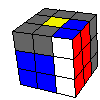
\includegraphics[height=20mm]{Rp.png} \hspace{1cm}} & \multirow{3}[3]{*}{R' \hspace{1cm}} & x-F & (U R' U) (R U2 R')
\\ \cmidrule{3-4}
& & x-L & R'
\\ \cmidrule{3-4}
& & F-L & U2 R' U' (R U' R')
\\ \bottomrule
\end{tabular}
\end{table}

\end{document}
